% PAKETE UND DOKUMENTKONFIGURATION
\documentclass[10pt, a4paper]{article}

% Encoding für Umlaute
\usepackage[utf8]{inputenc}

% Silbentrennung
\usepackage[ngerman]{babel}

% erweiterte Matheumgebungen
\usepackage{amsmath}

%
\usepackage{amsfonts}

%
\usepackage{amssymb}

% Einheiten setzen z.B. \SI{10}{\kilo\gram\meter\per\second\squared}
% Fehler: \SI{10 +- 0,2e-4}{\metre}
\usepackage{siunitx}
\sisetup{
  output-decimal-marker={,},
  separate-uncertainty
}

% Randbreiten
\usepackage[left=3cm,right=4cm,top=3cm,bottom=3cm,twoside]{geometry}

% Bilder einfügen
\usepackage{graphicx}

%Verwise innerhalb des Dokuments
\usepackage{hyperref}
\hypersetup{
	colorlinks = true,
	allcolors = {black}
}

%bessere Tabellenlayouts
\usepackage{booktabs}

% Tiefe des Inhaltsverzeichnisses (Level: 1 sections, 2 subsections,
% 3 subsubsections)
\setcounter{tocdepth}{2}

% DOKUMENTINFORMATIONEN
\title{P422 \\ Rastertunnelmikroskopie}

\author{Christopher Deutsch\footnote{christopher.deutsch@uni-bonn.de} \and Christian Bespin\footnote{christian.bespin@uni-bonn.de}}

\date{\today}

\begin{document}
  
\maketitle

% DURCHFÜHRUNGSDATUM UND ASSISTENT
\begin{center}
\begin{tabular}{l r}
Durchführung: & 20./21. Oktober 2014 \\
Gruppe: &$\alpha$ 2 \\
Assistent: & Peter Klassen
\end{tabular}
\end{center}

% ZUSAMMENFASSUNG
\begin{abstract}
% Text
\end{abstract}

% INHALTSVERZEICHNIS
\tableofcontents
% Neue Seite nach TOC
\newpage

% INHALT VERSUCHSPROTOKOLL
\section{Grundlagen}

\subsection{Tunneleffekt und Tunnelstrom}
Der Tunneleffekt ist ein quantenmechanisches Phänomen, welches einem einlaufenden Teilchen der Energie $E$ erlaubt, eine klassisch unüberwindbare Potentialschwelle der Höhe $V_0 > E$ mit endlicher Wahrscheinlichkeit zu durchqueren.
Im Gegensatz zum klassischen Fall, bei dem das Teilchen am Potentialwall reflektiert wird, nimmt bei der quantenmechanischen Beschreibung das Betragsquadrat der Wellenfunktion $|\Psi|^2$ und damit die Aufenthaltswahrscheinlichkeitdichte des Teilchens exponentiell mit der Eindringtiefe $s$ in den Wall ab.

Dieser Effekt wird beim Rastertunnelmikroskop (RTM) ausgenutzt, indem eine Spannung $U$ zwischen dem zu untersuchenden, leitenden Objekt und der ebenfalls leitenden Spitze des RTM angelegt wird.
Wenn nun die Spitze nah genug an die Probe gebracht wird, können die Elektronen durch die Potentialbarriere zwischen Spitze und Probe tunneln, was zu einem messbaren Tunnelstrom $I_\mathrm{T}$ führt.
Der Tunnelstrom für eine Potentialschwelle der mittleren Höhe $\Phi$ ist gegeben durch \cite{binning}:
\begin{equation}
  I_\mathrm{T} \propto \exp(-\alpha \cdot \sqrt{\Phi} \cdot s) \quad \text{mit}\: \alpha = \SI{1,025}{\angstrom^{-1}\electronvolt^{-1/2}}
  \label{eq:tunnelstrom}
\end{equation}
also abhängig vom Abstand Spitze-Probe $s$, sowie von deren elektronischen Eigenschaften.

Für kleine Spannungen $U$ ist die mittlere Höhe $\Phi$ gegeben durch die Austrittsarbeit des Elektrons aus dem Material \cite{colton}.
An Gleichung \ref{eq:tunnelstrom} erkennt man bereits die hohe Sensitivität auf Abstandsänderungen in der Größenordnung von einem \si{\angstrom}, weshalb das vorderste Atom auf der Spitze maßgeblich für den gemessenen Tunnelstrom ist.

\subsection{Funktionsweise des Rastertunnelmikroskops}
\subsubsection{Aufbau und Operation}
\begin{figure}[h]
\centering
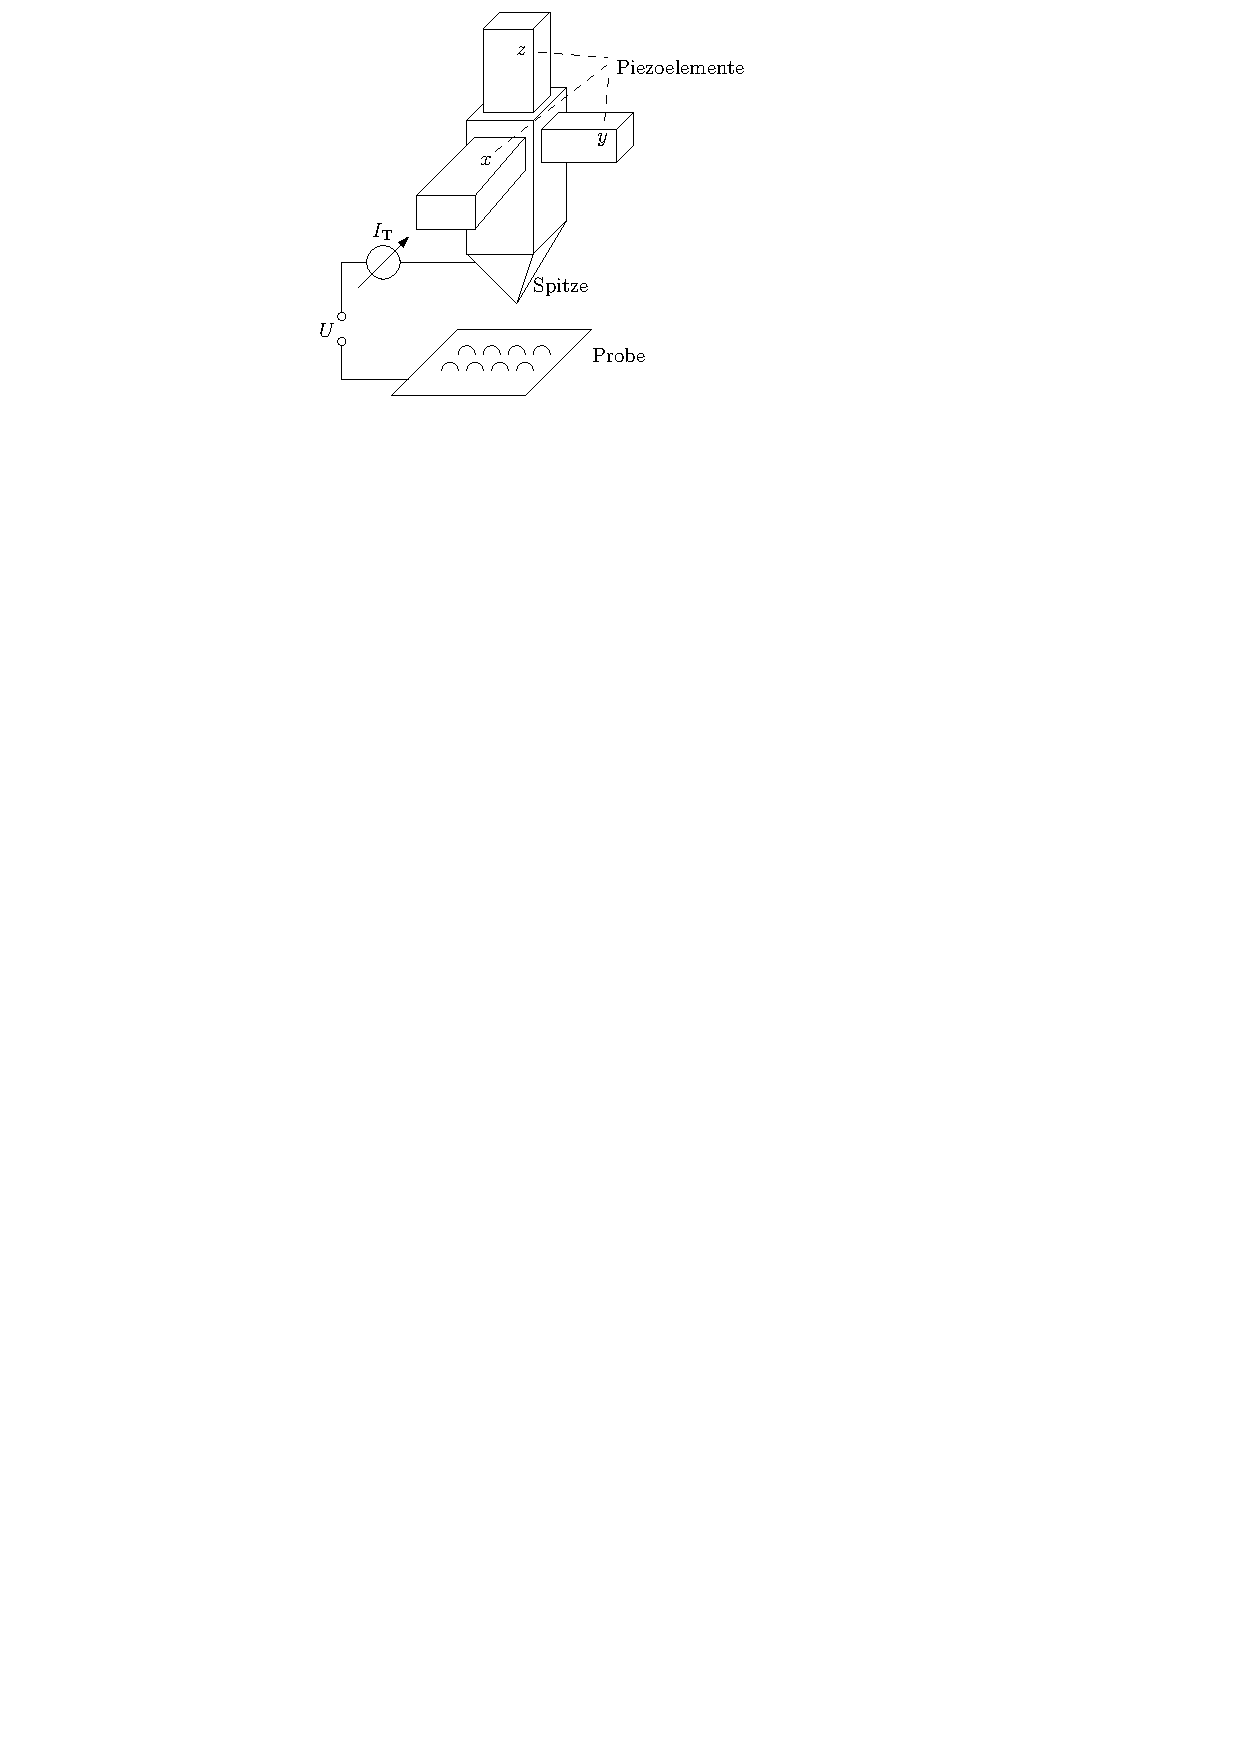
\includegraphics[width=0.5\textwidth]{./grafiken/rtm_aufbau.pdf}
\caption{schematischer Aufbau eines RTM mit Piezoelementen}
\label{fig:aufbau}
\end{figure}
Der Kern des Rastertunnelmikroskops (schematisch in Abbildung \ref{fig:aufbau}) ist die Rastersonde mit der aufgesetzten leitenden Spitze.
Diese kann über drei Piezoelemente (siehe auch \ref{sssec:Piezoeffekt}), deren Auslenkung proportional zu einer an ihnen anliegenden Spannung ist, räumlich bezüglich der Probe ausgerichtet werden.
Es werden Piezos verwendet, da die Spitze mit subatomarer Präzision eingestellt werden muss, um eine laterale und vertikale Auflösung im subatomaren Bereich zu erzielen.

Zwischen der Spitze der Sonde und der Probe liegt die Spannung $U$ an, damit bei ausreichender Annäherung ein messbarer Tunnelstrom entsteht.
Dazu muss die Probe zunächst durch eine Grobeinstellung hinreichend nah an die Spitze geführt werden.
Nachdem dies durchgeführt wurde, kann eine Feineinstellung über das z-Piezo erfolgen.

Zur Bildgebung durchläuft die Sonde mithilfe der x- und y-Piezoelemente eine gleichmäßig Verteilung von Messpunkten in der x-y-Ebene (das Raster), deren Dichte im Wesentlichen durch die eingestellte Auflösung und den Messbereich gegeben sind.
Die an den einzelnen Punkten gemessene Größe, sowie die Operation des z-Piezos hängt vom verwendeten Betriebsmodus des RTM ab und wird in Abschnitt \ref{sec:betriebsmodi} näher erläutert.


\subsubsection{Piezoeffekt}
\label{sssec:Piezoeffekt}
In Elementarzellen mit nicht-inversionssymmetrischer Ladungsverteilung kann, bei Deformation der Zelle durch eine externe Kraft, ein elektrisches Dipolmoment, durch die Verschiebung des positiven und negativen Ladungsschwerpunkts, induziert werden.
Das durch die Polarisation entstandene elektrische Feld lässt sich als Spannung an den Oberflächen von piezoelektrischen Materialien messen.
\begin{figure}[h]
\centering
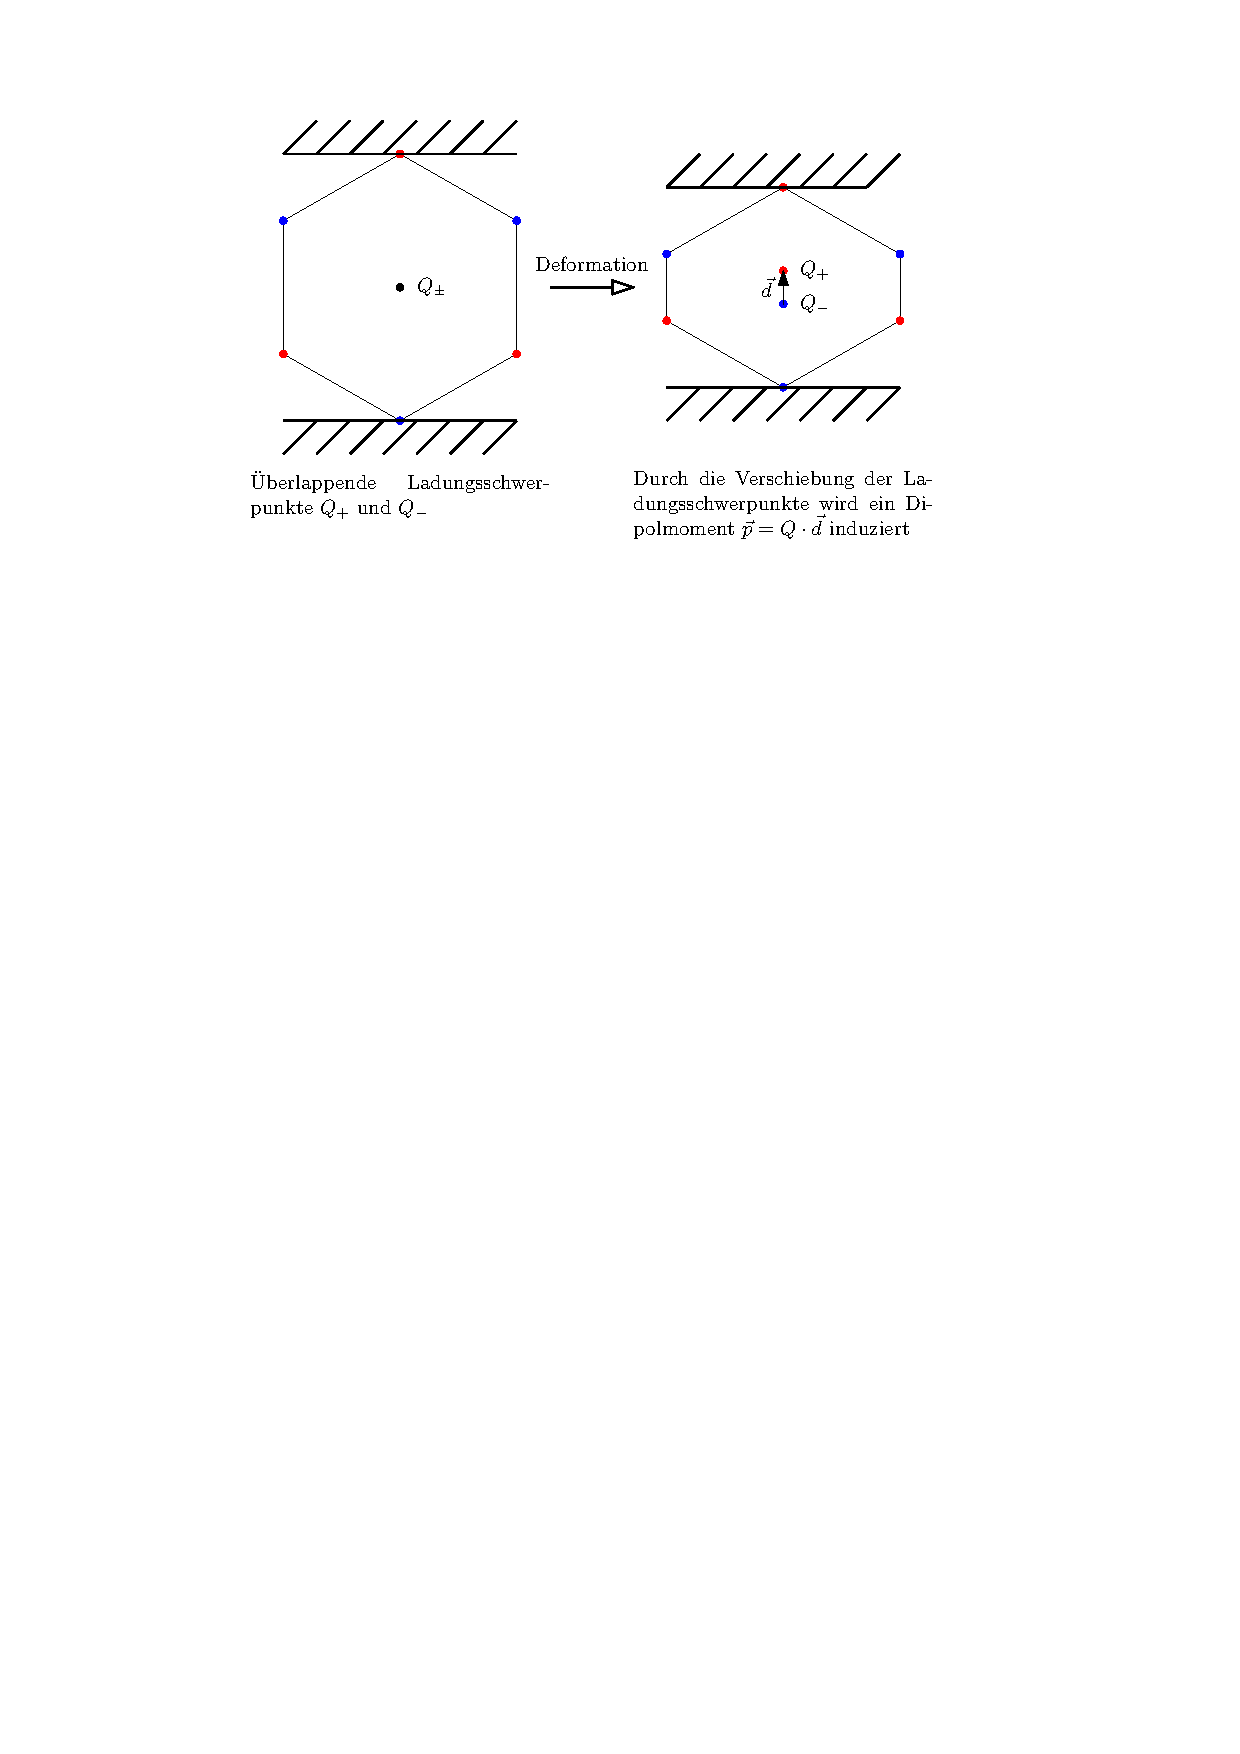
\includegraphics[width=0.8\textwidth]{./grafiken/piezoeffekt.pdf}
\caption{induziertes Dipolmoment bei Deformation einer nicht-inversionssymmetrischen Ladungsverteilung}
\end{figure}

Umgekehrt kommt es beim Anlegen einer Spannung an einem piezoelektrischen Kristall zur Polarisation dessen und durch diese zur Deformation des Kristalls aufgrund der Asymmetrie der Ladungsverteilung.
Dieser Effekt führt bei makroskopischen Objekten zu einer sehr kleinen Längenänderung bei angelegter Spannung und ist daher besonders für die präzise Steuerung innerhalb eines kleinen Bereichs geeignet.

\subsubsection{Betriebsmodi}
\label{sec:betriebsmodi}
Wir gehen im Folgenden davon aus, dass wir die Spannung zwischen Spitze und Probe in beiden Fällen konstant lassen.
Dann sind im Betrieb eines Rastertunnelmikroskops grundsätzlich zwei Betriebsmodi zu unterscheiden:
\begin{itemize}
  \item \textbf{konstanter Tunnelstrom:} Dieser wird erreicht, indem der Tunnelstrom an jedem Punkt gemessen wird und durch eine Rückkopplungsschleife (siehe auch Abschnitt \ref{sssec:Regelkreis}) die Höhe der Spitze so eingestellt wird, dass der Tunnelstrom einen konstanten, vorgegebenen Wert annimmt.
Die Bildgebung erfolgt durch Darstellung der anliegenden Spannung am z-Piezo, welche proportional zur Ladungsdichte ist, da sich die Spitze des RTM, aufgrund des konstanten Tunnelstroms, in der Ebene konstanter Ladungsdichte bewegt.
Weiterhin sorgt die Reaktionszeit des Regelkreises dafür, dass das Verfahren im Vergleich zum Betriebsmodus mit konstanter Höhe deutlich langsamer ist, jedoch die Gefahr eines Zusammenstoßes von Spitze und Probe unterbunden wird.

  \item \textbf{konstante Höhe:} Die Spitze des RTM bewegt sich mit einer festgelegten und konstanten Höhe über die Probe.
Die eigentliche Messgröße ist dabei der fließende Tunnelstrom, welcher ebenfalls Rückschlüsse auf die elektronische Struktur der Probe liefert.
Da außer der Rasterbewegung der Spitze keine weiteren Regelungen notwendig sind, ist dieses Verfahren geeignet, um in kurzer Zeit Bilder der Probe zu erhalten, allerdings besteht dabei die Gefahr einer Kollision, bei der die Spitze in die Probe fährt und dadurch zerstört wird.

Dieser Betriebsmodus ist also für flache Strukturen der Probe mit einer durchschnittlichen Höhe kleiner als der Abstand Probe-Spitze geeignet \cite{colton}.
Da es praktisch kaum möglich ist, vertikale Verschiebungen auszuschließen und die Probe nicht immer parallel zur horizontalen Bewegung der Spitze ausgerichtet ist, wird auch hier eine Rück\-kopp\-lungs\-schlei\-fe, wie oben erklärt, verwendet, allerdings mit einer geringen Empfindlichkeit. Dadurch ist sichergestellt, dass die Spitze nicht auf schnelle Änderungen des Tunnelstroms reagiert, aber langfristig eine vorgegebene Höhe über der Probe (auch wenn diese gegen die horizontale Bewegungsebene der Spitze geneigt ist) erreicht wird.
\end{itemize}
Neben diesen beiden gibt es noch Betriebsmodi bei denen der Abstand Spitze-Probe an jedem Punkt variiert wird, um die Austrittsarbeit zu bestimmen \cite{sakai}.
Außerdem können durch eine Variation der Spannung zwischen Probe und Spitze weitere elektronische Eigenschaften der Probe bestimmt werden (\emph{Rastertunnelspektroskopie}).

\subsubsection{Regelkreis}
\label{sssec:Regelkreis}
Wie im vorigen Abschnitt angesprochen, dient der Regelkreis dazu, einen konstanten Tunnelstrom über dem Messbereich zu erhalten.
Dafür muss dieser kontinuierlich gemessen und über einen Strom-Spannungswandler mit Verstärker in eine proportionale Spannung gewandelt werden.
Nun muss die Spannung am z-Piezo und damit die Höhe der Spitze so eingestellt werden, dass der Tunnelstrom (bzw. die proportionale Spannung) einen fest vorgegebenen Wert annimmt.

Diese Funktion wird von sogennanten Reglern ausgeführt, welche ein Eingangssignal mit einem Referenzwert vergleichen und anhand Eingangssignal und Referenzwert ein Ausgangssignal erzeugen (die genaue Abhängigkeit hängt vom Typ des Reglers ab).
Ein solcher Regler wird durch eine Rückkopplung einer vom Ausgangssignal abhängigen Größe (hier regelt das Ausgangssignal die Höhe der Spitze und hat damit ebenfalls einen Einfluss auf den Tunnelstrom, welcher als proportionale Spannung am Eingang liegt) auf den Eingang zu einem Regelkreis verbunden.

Je nach Anwendungsfall werden verschiedene Reglertypen mit jeweils unterschiedlichen Eigenschaften verwendet.
So genannte \emph{P-Regler} liefern ein zur Eingangsgröße proportionales Signal mit einer festen Verstärkung.
In der Praxis werden solche Regler meist um eine integrierende und/oder differenzierende Funktion erweitert. Entsprechend spricht man dann beispielsweise von \emph{PI-} oder \emph{PID-Reglern}.
Der integrierende Teil sorgt für eine zeitabhängige Schaltung, so dass auch die Eingangsgröße eine gewisse Zeit in der Vergangenheit überwacht wird (\emph{Hysterese}) und daraufhin ein entsprechendes Schaltverhalten eintritt.
Der differenzierende Teil hingegen reagiert nicht auf den Wert des Eingangssignals sondern auf Änderungen dessen.

\subsubsection{Auflösungsvermögen}
Man sieht bereits an Gleichung \ref{eq:tunnelstrom} dass die Tiefenauflösung des RTM bei typischen Austrittsarbeiten $\Phi = \SI{4}{\electronvolt}$ idealerweise in der Größenordnung von \SI{0,1}{\angstrom} liegt.
Die laterale Auflösung hingegen ist stark abhängig von der Struktur der Spitze und liegt für brauchbare Spitzen in der Größenordnung von \SI{1}{\angstrom}.

\subsection{Spitzenherstellung}
Um ein möglichst hohes Auflösungsvermögen zu erreichen, ist eine dünne Spitze (idealerweise ein einzelnes Atom) nötig.
Im Folgenden werden zwei Spitzenherstellungsmethoden angesprochen, dabei wird die konkrete Vorgehensweise im Abschnitt Versuchsdurchführung erläutert.

\begin{itemize}
\item \textbf{mechanisches Reißen:} Bei dieser Methode wird ein Stück Draht ruckartig zerrissen, wodurch an der gerissenen Stelle manchmal eine Spitze mit einer Breite von wenigen Atomen entsteht.
Da die Form  der so entstandenen Spitzen nicht vorherzusehen ist, kann es dazu führen, dass mehrere atombreite Herausragungen entstehen, welche bei der Bildgebung zu sogenannten Geisterbildern (parallele Strukturen durch Mehrfachspitzen) führen.

\item \textbf{elektrochemisches Ätzen:} Ein Draht wird in ein geeignetes Elektrolyt eingetaucht und mit dem positiven Pol einer Spannungsquelle verbunden.
Der negative Pol der Spannungsquelle wird mit einer Elektrode im Elektrolyt verbunden.
Bei anliegender Spannung können Metallionen des Drahtes in das Elektrolyt übergehen und von der Drahtoberfläche abgetragen werden.
Um die Ätzwirkung besser zu lokalisieren kann die Form der Elektrode so gewählt werden, dass der Draht an gewissen Stellen stärker abgetragen wird.
Der Ätzprozess wird solange fortgesetzt, bis eine Stelle des Drahtes so dünn geworden ist, dass der untere Teil abbricht.
Dann sollte die Spannungquelle ausgeschaltet werden und der Draht aus dem Elektrolyt entfernt werden, um ein Abstumpfen der Spitze zu vermeiden.
Diese Methode liefert tendenziell besser definierte Spitzen als das mechanische Reißen.
\end{itemize}

\subsection{Kristallstruktur von Graphit}
\label{ssec:graphit}
\begin{figure}[h]
  \centering
  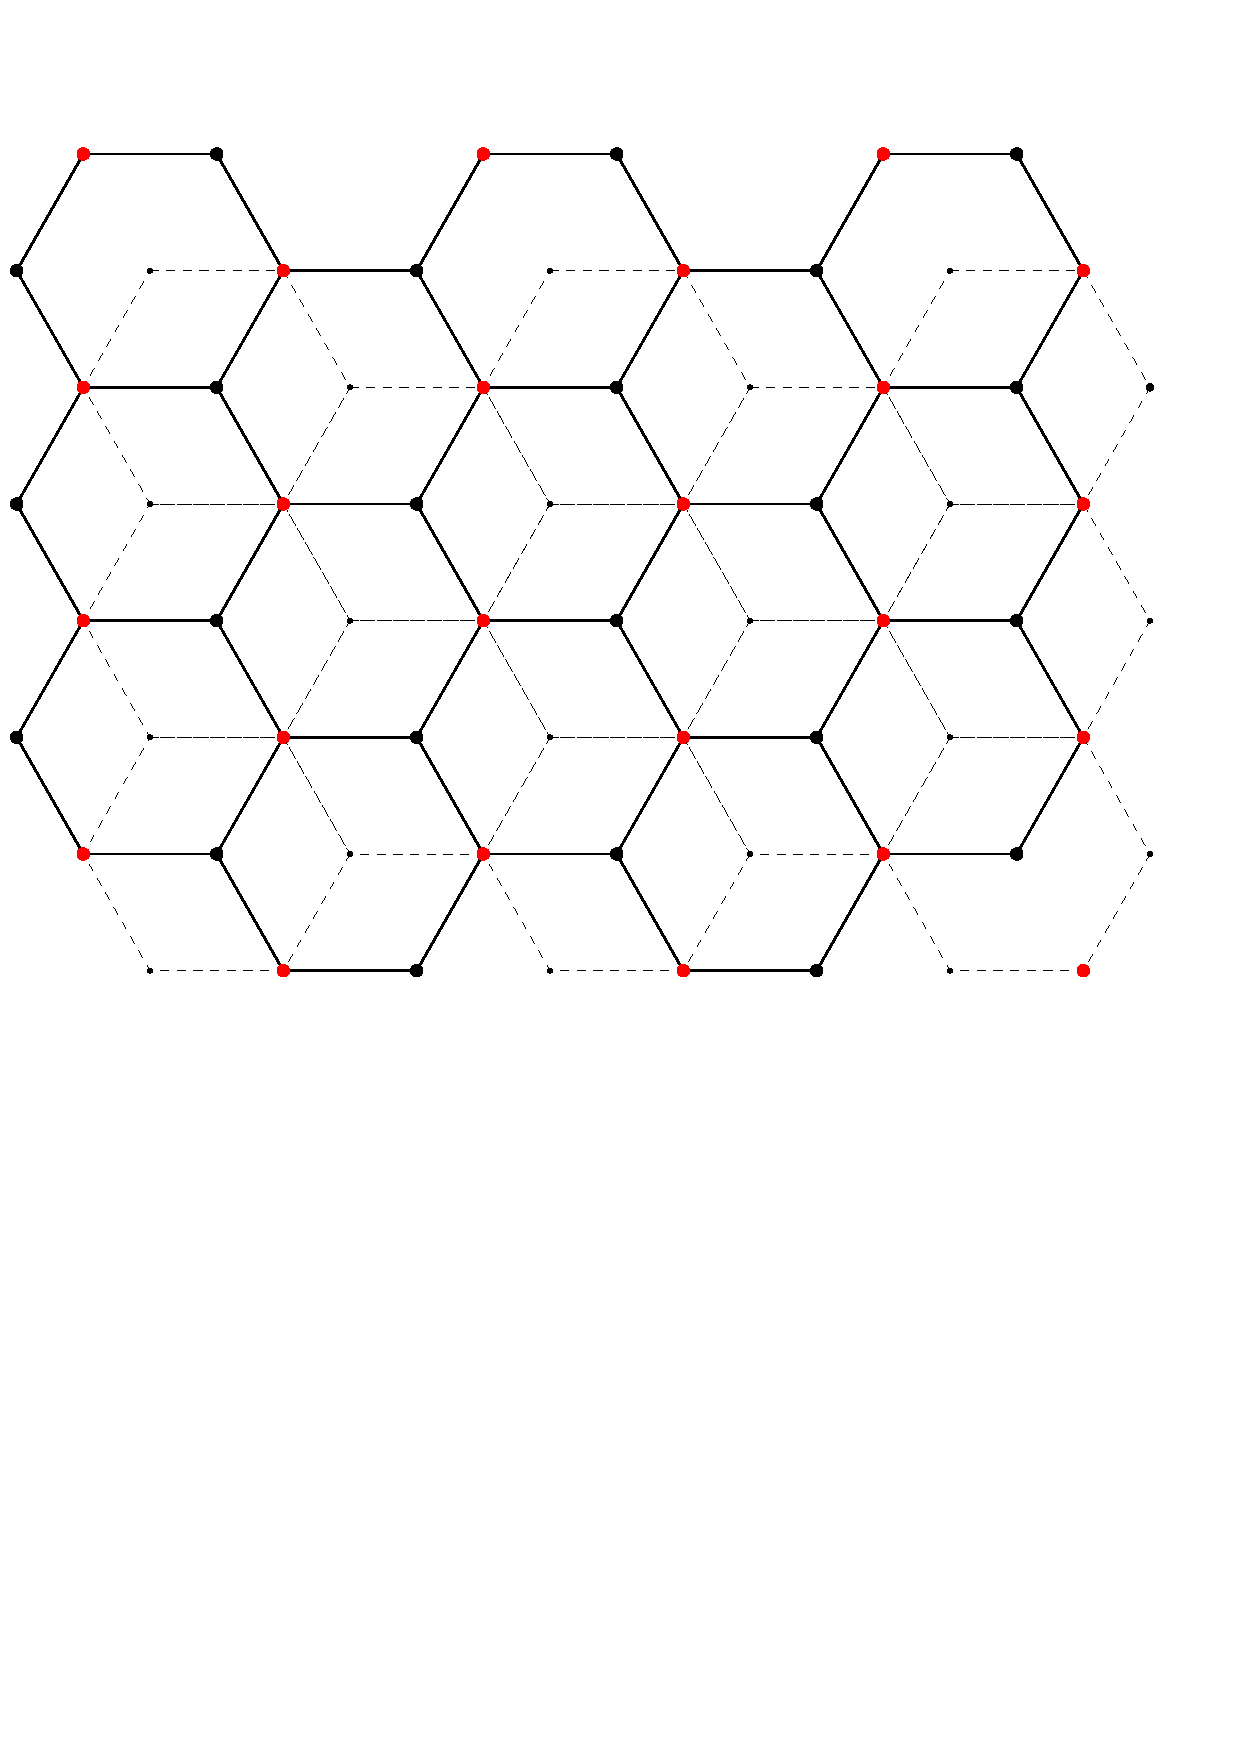
\includegraphics[width=0.6\textwidth]{grafiken/graphit.pdf}
  \caption{Schematische Darstellung der obersten zwei Ebenen eines Graphit-Kristalls. Die Kohlenstoffatome, die in der oberen (fett) und der unteren Ebene (gestrichelt) überlappen sind in rot markiert.}
  \label{fig:graphit}
\end{figure}
Graphit besteht aus planen Kohlenstoffebenen mit einer regelmäßigen hexagonalen Struktur, wobei der Abstand der Kohlenstoffatome \SI{1,42}{\angstrom} \cite{colton} und der Bindungswinkel \SI{120}{\degree} beträgt.
Diese Ebenen liegen unter einem solchen Versatz übereinander, der das Zentrum eines Hexagons mit einem Kohlenstoffatom in der darunterliegenden Ebene zusammenfallen lässt (Abbildung \ref{fig:graphit}).

Aufgrund des Einflusses der überlappenden Kohlenstoffatome (in der Abbildung rot) auf die Ladungsdichte an der Oberfläche, sind diese nur als Täler bei der Bildgebung zu erkennen, wohingegen die nicht-überlappenden Atome als Berge sichtbar sind.
Aus diesem Grund ist der Abstand der bei der Rastertunnelmikroskopie sichtbaren Ladungsdichtenmaxima:
\begin{equation*}
d_\mathrm{max} = 2 \cdot \SI{1,42}{\angstrom} \cdot \sin\left( \frac{1}{2} \cdot 120\si{\degree} \right) = \SI{2,46}{\angstrom}
\end{equation*}

\subsection{Verwandte Rastermethoden}
\begin{itemize}
  \item \textbf{Rasterkraftmikroskopie:} Um nicht-leitende Oberflächen zu untersuchen ist die Rastertunnelmikroskopie ungeeignet.
  Stattdessen nutzt man die interatomaren Kräfte zwischen dem Objekt und einer Blattfeder mit dünner Spitze aus, um aus deren Auslenkung das Profil der Oberfläche zu bestimmen.
  Ähnlich zum RTM gibt es im Kontaktbetrieb des Rasterkraftmikroskops zwei typische Betriebsmodi:
  \begin{itemize}
  \item[--] konstante Kraft: Eine Rückkopplungsschleife zwischen Auslenkungsmessung und Höheneinstellung sorgt dafür, dass die Auslenkung und damit die Kraft konstant gehalten wird.
  So ist das Profil des Objektes gegeben durch die Blattfederhöhe.
  \item[--] konstante Höhe: Die Höheneinstellung bleibt unverändert und das Profil des Objektes ist gegeben durch die Auslenkung der Feder.
  \end{itemize}
  Es gibt bei der Rasterkraftmikroskopie noch weitere Betriebsmodi auf die an dieser Stelle aber nicht weiter eingegangen wird.
\end{itemize}

\section{Versuchsdurchführung}
\label{sec:durchfuehrung}

In dem Versuch sollten geeignete Spitzen zum Abbilden von Graphitoberflächen hergestellt werden und anschließend mit ihnen auf atomarer Ebene Bilder der Oberfläche aufgenommen werden.
Für Graphit sollten dabei Eigenschaften des Kristallgitters, wie Atomabstände und Winkel der Bindungen untersucht und aus den Bildern bestimmt werden. 
Außerdem sollte mit einer Spitze, die bei Graphit atomare Auflösung erreicht, eine Goldoberfläche abgebildet werden und diese mit dem vorigen Bild verglichen werden.

\subsection{Herstellung der Spitzen}

\subsubsection{Reißen der Platin-Iridium Spitzen}

Zur Herstellung der Pt-Ir Spitzen wird ein kurzes Stück Draht zunächst mit Ethanol gereinigt und dann mit einer Zange festgehalten, so dass das andere Ende mit einem Seitenschneider im spitzen Winkel gepackt werden kann.
Dabei ist darauf zu achten, dass man mit dem Seitenschneider nicht schneidet, sondern den Draht nur festhält.
Nun wird ruckartig und longitudinal Druck ausgeübt, so dass der Draht abreißt. Idealerweise ist dann schon eine geeignete Spitze entstanden, die direkt in das RTM eingesetzt werden kann.

Das Reißen gelang mit etwas Übung recht gut, obwohl dabei keine gute Spitze produziert werden konnte.

\subsubsection{Ätzen der Wolfram Spitzen}
Bei den Wolfram Spitzen muss grundsätzlich bedacht werden, dass Wolfram an Luft schnell oxidiert. 
Darum ist vor dem Ätzvorgang die Oxidschicht mit Schleifpapier zu entfernen und  der Draht mit Ethanol zu reinigen.
Der Draht wird dann in der Ätzvorrichtung einige Millimeter in Kalilauge (Kaliumhydroxid mit Konzentration \SI{2}{\mol\per\cubic\deci\metre}) getaucht.
\begin{figure}[h]
\centering
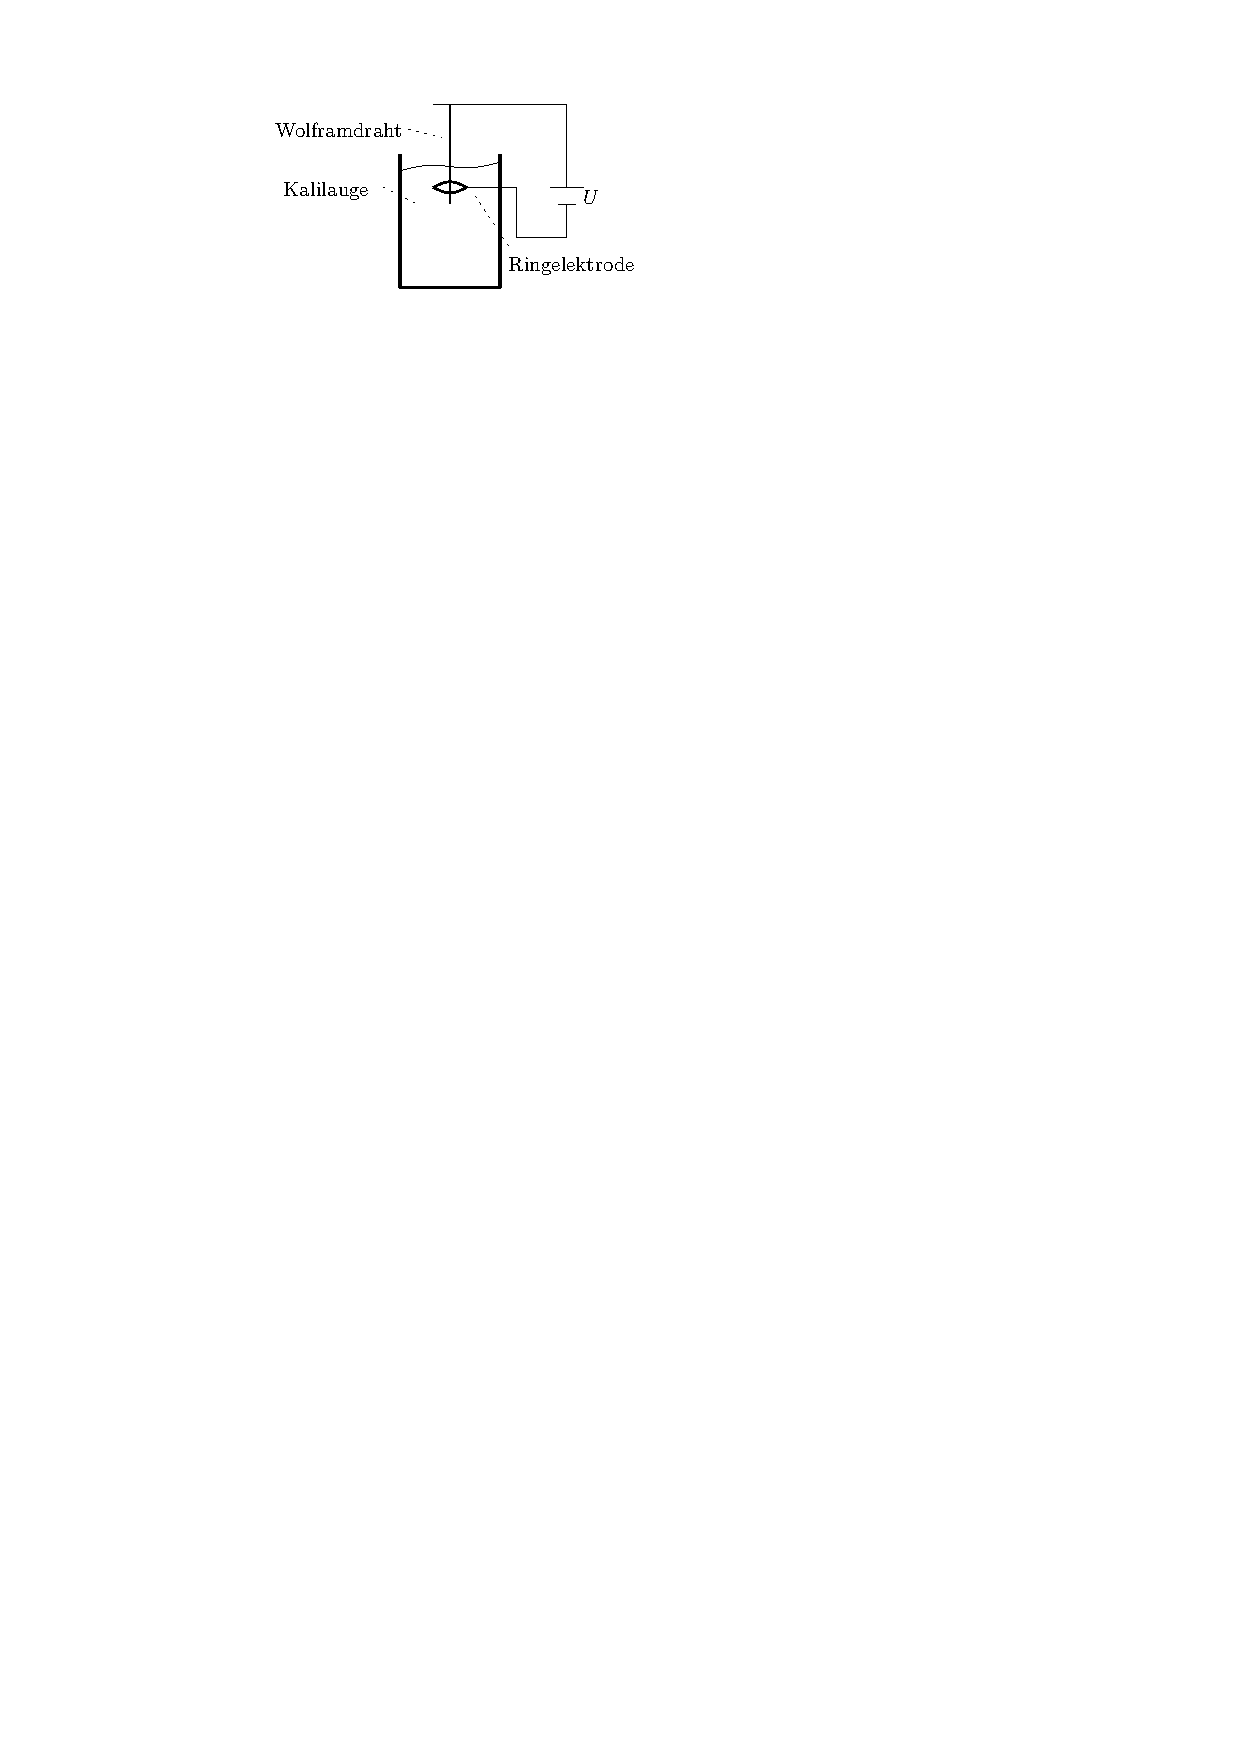
\includegraphics[width=0.4\textwidth]{./grafiken/aetzvorrichtung.pdf}
\caption{Ätzvorrichtung zur Herstellung der Wolframspitzen}
\label{fig:aetzen}
\end{figure}
Knapp unterhalb der Kalilaugenoberfläche befindet sich eine Ringelektrode um die Ätzwirkung zu lokalisieren.
Zwischen Wolframdraht (Anode) und Ringelektrode wird eine Spannung von \SI{10}{\volt} angelegt, sodass sich Wolframionen aus dem Draht nahe der Wolframdraht--Kalilauge--Luft-Grenzschicht lösen können und zur Elektrode wandern.
Nun wird der Stromfluss beobachtet um den Moment abzupassen, an dem der Draht am Meniskus bricht.
Dies wird durch den schnellen Abfall des fließenden Stroms angekündigt, da der Querschnitt des Drahtes nun sehr klein ist.

Entgegen der Information aus der Praktikumsanleitung war dieser Effekt nicht zu beobachten, der Strom fiel die ganze Zeit über nur sehr langsam (ein Ätzvorgang ca. \num{20}--\SI{30}{\minute}) ab.
Weiterhin brach der Draht nicht am Meniskus, sondern irgendwo in der Lauge ab.  
Nach dem Ätzen ist die Spitze erneut zu reinigen und zügig zu arbeiten, um einer Oxidation der Spitze zu vermeiden.

\subsection{Handhabung von Probe und Spitze}

Da das Rastertunnelmikroskop mit sehr feinen Mechaniken und Auflösungen auf atomarer Ebene arbeitet, ist ein besonders sorgfältiger, sauberer Umgang mit allen Teilen notwendig.
Die Geräte wie Zangen, Pinzetten, aber auch die Drähte sollten vor der Verarbeitung immer mit Ethanol gereinigt werden.
Ebenfalls sollte die Mechanik des RTM, also die Führungsschiene für den Probenhalter und der Probenhalter selber sauber gehalten werden, damit dieser ungehindert von dem Piezoelement zur Grobeinstellung bewegt werden kann.

Diese Grobeinstellung erfolgt über den \emph{Slip-Stick-Effekt}, welcher ausnutzt, dass Haftreibung tendenziell größer ist als Gleitreibung und so durch eine langsame Ausdehnung des Piezos die Probe vorschiebt.
Ein ruckartiges Kontrahieren aufgrund der geringeren Gleitreibung und der Trägheit des Halters ruft allerdings keine Positionsänderung hervor.
Deshalb ist die Reinigung des Probenhalters kritisch, wie im Versuch mehrfach festgestellt wurde.

\subsection{Datenaufnahme}

Nach dem erfolgreichen Einsetzen von Probe und Spitze kann versucht werden, Daten aufzunehmen.
Beim Einsetzen der Spitze ist zu beachten, dass diese nicht übermäßig lang ist, da sonst die Probe so weit hinten positioniert werden muss, dass der Stellmotor (\emph{Slip-Stick}-Piezo) ihn nicht mehr bewegen kann.
Nun wird zunächst per Hand der Probenhalter möglichst nah an die Spitze bewegt und dann im Computerprogramm mit \textit{Advance} schrittweise näher herangefahren.
Der Abstand ist dabei mit einer in der Abdeckung des RTM eingebauten Lupe zu kontrollieren.
Ist die Probe möglichst nah positioniert (die Kontroll-LED im Programm und auf dem Gerät sollte orange leuchten), kann mit \textit{Approach} im Computerprogramm eine automatische Annäherung mit dem z-Piezoelement gestartet werden.
Dies gelingt nicht immer, dann muss erneut manuell korrigiert und ein weiterer Annäherungsversuch gestartet werden.
Ist die Annäherung abgeschlossen, leuchtet die LED grün und es beginnt automatisch die Datennahme mit den eingestellten Parametern (zu rasternde Fläche, angestrebter Tunnelstrom etc.).

Nach mehreren Versuchen pro Spitze gelang es meistens, eine laut Software gute Annäherung zu erreichen, wobei die Spitze, mit bloßem Auge erkennbar, bei einigen Durchgängen trotzdem noch weit von der Probe entfernt war.
Teilweise konnte auch gar keine Annäherung durchgeführt werden, so dass die Kontroll-LED von orange direkt auf rot sprang, was bedeutet, dass die Spitze in die Probe gefahren ist.
Ein weiterer Störfaktor sind Erschütterungen in dem Versuchsraum, hauptsächlich ausgelöst durch die im Nebenraum befindliche Werkstatt, deren Maschinen spürbare Erschütterungen des Tisches hervorriefen.

\section{Messdaten}
Wir konnten leider keine verwertbaren Messergebnisse erzielen und verwenden daher die bereitgestellten Referenzbilder zur quantitativen Auswertung.
Eine genauere Erläuterung der Störfaktoren wird in Abschnitt \ref{sec:Diskussion} gegeben.

\subsection{Messung der Graphitoberfläche mit einer gerissenen Pt-Ir Spitze}
\begin{figure}[!h]
\centering
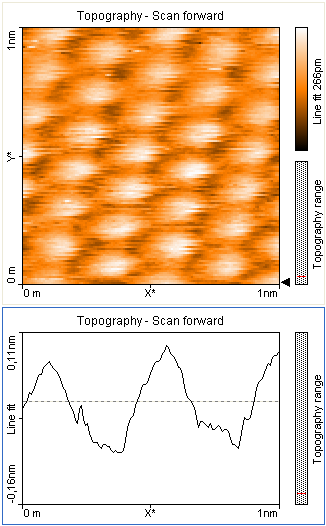
\includegraphics[width=0.5\textwidth]{./grafiken/originale/ref_graphit_pt_ir_1nm.png}
\caption{Aufnahme einer Graphitoberfläche mit einer gerissenen Pt-Ir Spitze (Referenzbild)}
\label{fig:ref_ptir}
\end{figure}

In der Aufnahme sind deutlich die für Graphit erwarteten Ergebnisse zu sehen.
So finden wir an den hellen Stellen die alleinstehenden Atome der oberen Gitterebene und sehen an den dunklen Stellen den Überlapp der Atome in der oberen und unteren Ebene, die wie in Abschnitt \ref{ssec:graphit} beschrieben, dazu führen, dass dort die Ladungsdichte geringer ist.
Außerdem sieht man eine Verzerrung des Bildes, worauf in Abschnitt \ref{ssec:laenge} bei der Bestimmung der Bindungslänge näher eingegangen wird.

\subsection{Messung der Graphitoberfläche mit einer geätzten W Spitze}
\begin{figure}[!h]
\centering
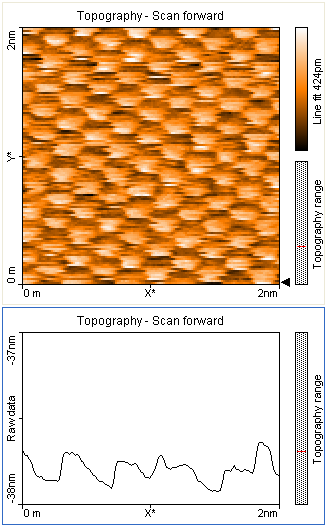
\includegraphics[width=0.5\textwidth]{./grafiken/originale/ref_graphit_w_2nm.png}
\caption{Aufnahme einer Graphitoberfläche mit einer geätzten Wolfram Spitze (Referenzbild)}
\label{fig:ref_w}
\end{figure}

Die Maxima sind in dieser Aufnahme nicht zu erkennen.
Die hier genutzte Wolframspitze ist außerdem offensichtlich nicht von genügender Qualität, um größere Vergrößerungen zu messen; bereits bei dieser Bildgröße ist keine Struktur mehr erkennbar.

\subsection{Messung einer Goldoberfläche}
Die uns zur Verfügung stehenden Referenzbilder für Messungen einer Goldoberfläche sind leider alle nicht gut auszuwerten, da die dort genutzten Messbereiche nicht vergleichbar mit denen in den Messungen von Graphit sind.
Zudem ist die Kristallstruktur von Gold grundsätzlich schwieriger darzustellen, da Gold eine homogenere Ladungsdichte als Graphit hat.
Es sind daher nicht so deutliche Berge und Täler wie bei Graphit zu sehen. 

\section{Auswertung}
Die folgende quantitative Auswertung beschäftigt sich mit der Bestimmung der Vergrößerung des Rastertunnelmikroskops sowie einiger Kenngrößen der zugrundeliegenden Graphitstruktur wie der Bindungslänge und dem Bindungswinkel der hexagonalen Kohlenstoffringe.

\subsection{Bestimmung der Vergrößerung des Mikroskops}
Zur Bestimmung der Vergrößerung von Abbildung \ref{fig:ref_ptir} ist zunächst anzumerken, dass das Seitenverhältnis von Abbildung und Messbereich $1:1$ ist, sodass die Vergrößerung in $x$- und $y$-Richtung gleich ist ($V_x = V_y$). Außerdem hängt die Größe des Bildes von der Vergrößerungsstufe im Computerprogramm bzw. der Größe des Ausdrucks ab. Als Referenzwert werden wir die Größe des Ausdrucks der Abbildung \ref{fig:ref_ptir} in diesem Protokoll verwenden, sodass sich die Vergrößerung ergibt als:
\begin{equation}
  V = V_x = \frac{L_x}{l_x}
\end{equation}
wobei wir $L_x$ als x-Kantenlänge des Ausdrucks und $l_x$ als Größe des Messbereichs in x-Richtung definieren.
Der Fehler folgt aus Gauß'scher Fehlerfortpflanzung:
\begin{equation}
  \Delta V = \sqrt{\frac{\Delta L_x ^2}{l_x^2} + \frac{L_x^2 \cdot \Delta l_x^2}{l_x^4}}
\end{equation}
Die ausgedruckte Kantenlänge der Abbildung \ref{fig:ref_ptir} wird mit einem Lineal gemessen:
\begin{equation*}
  L_{x,\mathrm{Abb.\ref{fig:ref_ptir}}} = \SI{55 +- 0,5}{\milli\metre}
\end{equation*}
Wir nehmen auf dem Messbereich einen relativen Fehler von \SI{1}{\percent} an und erhalten:
\begin{align*}
  l_{x,\mathrm{Abb.\ref{fig:ref_ptir}}} = \SI{1,00 +- 0,01}{\nano\metre}
\end{align*}
Mit diesem Wert erhalten wir für die Vergrößerung des RTM:
\begin{align*}
  V_\mathrm{Abb.\ref{fig:ref_ptir}} = \num{55,0 +- 0,75e6}
\end{align*}
Zum Vergleich liegt die beugungsbegrenzte Vergrößerung für Lichtmikroskopie im optischen Bereich bei etwa $V_\mathrm{max}^\mathrm{Mikr.} \approx \num{1500}$, sodass wir mit dem RTM etwa die \num{37000}-fache Vergrößerung vom Lichtmikroskop an der Beugungsgrenze erreichen.

\subsection{Bestimmung der Bindungslängen in Graphit}
\label{ssec:laenge}
\begin{figure}[!h]
\centering
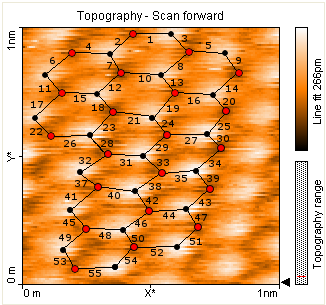
\includegraphics[width=0.5\textwidth]{./grafiken/laenge.png}
\caption{Konstruktion der hexagonalen Kohlenstoffringe im Bild des RTM aufgenommen mit einer Pt-Ir Spitze. In den zwei oberen Ebenen überlappende Kohlenstoffatome sind in rot markiert. Die Zahlen dienen der Linienidentifikation in Tabelle \ref{tab:laengen} im Anhang.}
\label{fig:laengen}
\end{figure}
Um die Bindungslängen zu bestimmen, müssen wir zunächst die hexagonale Ringstruktur der obersten Graphenebene bestimmen.
Da wir bei Vermessung der hexagonalen Struktur möglichst hohe Vergrößerung brauchen, verwenden wir das Ergebnis der Messung mit Pt-Ir Spitze da diese einen kleinen Messbereich von $\SI{1}{\nano\metre} \times \SI{1}{\nano\metre}$ aufweist.

Zunächst werden die nicht-überlappenden Kohlenstoffatome markiert, da diese als Erhebungen bei der Bildgebung sichtbar werden.
Gemäß Abschnitt \ref{ssec:graphit} werden die in den zwei obersten Ebenen überlappenden Kohlenstoffatome als Täler im Bild sichtbar, sodass auch diese markiert werden können.
Verbindet man nun die eingezeichneten Punkte zu hexagonalen Ringen (im Hinblick auf Abbildung \ref{fig:graphit}), so erhalten wir Abbildung \ref{fig:laengen}.

In der Abbildung sieht man deutlich, dass die Ebene der Probe nicht mit der $(x,y)$-Ebene des RTM zusammengefallen ist, da die Bindungslängen in manche Richtungen stark gestaucht sind.
Dies liegt daran, dass wir aufgrund des Darstellungstyps (\emph{Density Plot}) mit den eingezeichneten Linien nur die Projektion der Bindung in die $(x,y)$-Ebene des RTM erhalten.

Wir Bestimmen die Längen der eingezeichneten Linien mit einem Grafikprogramm, wobei wir den Fehler der digitalen Längenbestimmung vernachlässigen, da dieser klein gegen die Verzerrung des Bildes ist.
Die gemessenen Längen finden sich in Anhang \ref{messw:laenge}.

Um den systematischen Fehler aufgrund der Projektion (tendenzielle Unterschätzung der Bindungslänge) zu verringern, streichen wir zunächst die Messwerte von Bindungen, die in der Abbildung nach links-oben zeigen\footnote{Liniennummern: $3,7,9,11,13,18,20,22,24,28,30,33,37,39,42,45,47,50,53$}, da diese die größte Stauchung aufgrund von Projektion aufweisen.
Die bleibenden $N = \num{35}$ Längen können dann zur Bestimmung der Bindungslänge ausgewertet werden, wobei immernoch mit einer Unterschätzung des tatsächlichen Wertes zu rechnen ist.

Zunächst bestimmen wir die mittlere Bindungslänge durch das arithmetische Mittel und erhalten:
\begin{equation}
  \bar{d}_\mathrm{Bind.} = \frac{1}{N} \sum_{i=1}^N d_i= \SI{1,37}{\angstrom}
\end{equation}
Der Fehler einer Einzelmessung ist dabei gegeben durch die Standardabweichung:
\begin{equation}
  \sigma_\mathrm{d} = \sqrt{\frac{1}{N-1} \sum_{i=1}^N (d_i - \bar{d}_\mathrm{Bind.})^2} = \SI{0,15}{\angstrom}
\end{equation}
und folglich der Fehler des Mittelwerts als:
\begin{equation}
  \Delta \bar{d}_\mathrm{Bind.} = \frac{\sigma_\mathrm{d}}{\sqrt{N}} = \SI{0,03}{\angstrom}
\end{equation}
Wir erhalten also als Bindungslänge:
\begin{equation}
  d_\mathrm{Bind.} = \SI{1,37 +- 0,03}{\angstrom}
\end{equation}
Wie erwartet, unterschätzt dieses Ergebnis den in \cite{colton} gegebenen Wert für den Abstand der Kohlenstoffatome von \SI{1,42}{\angstrom}. Dennoch liegt der Literaturwert innerhalb des $2\sigma$-Bereichs unserer Messung, sodass unsere Bestimmung der Bindungslänge akzeptabel ist.

\subsection{Bestimmung der Bindungswinkel in Graphit}
\begin{figure}[hp]
\centering
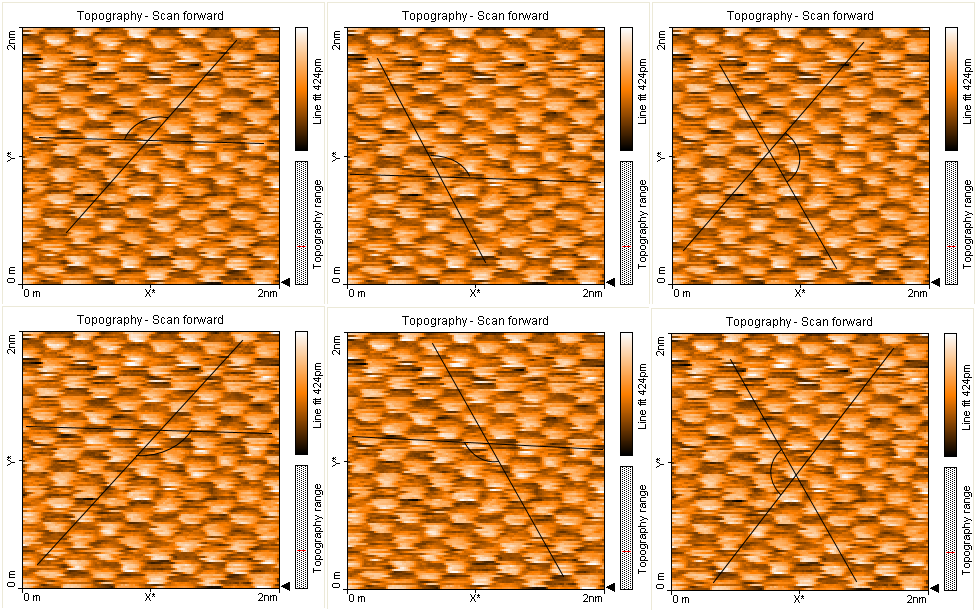
\includegraphics[width=1\textwidth]{./grafiken/collage.png}
\caption{Hilfsgeraden zur Bestimmung der Bindungswinkel}
\label{fig:hilfsgeraden}
\end{figure}
Zur Bestimmung des Bindungswinkels legen wir für jede Winkelmessung zwei Hilfsgeraden durch die Maxima des Bildes (siehe Abbildung \ref{fig:hilfsgeraden}).
Nach dem Vergleich mit den Abbildungen \ref{fig:graphit} und \ref{fig:laengen} liegt es nahe, dass es sich bei dem durch die Geraden eingeschlossenen Winkel um den jeweiligen Bindungswinkel handelt.
Weil man die Hilfsgeraden besonders gut bei kleinerer Vergrößerung einzeichnen kann, da man sich an mehreren Maxima orientieren kann, verwenden wir die Aufnahme der Graphitoberfläche mit der Wolfram Spitze, welche einen breiteren Messbereich von \SI{2}{\nano\metre} hat.
Insbesondere ist die Darstellung winkelerhaltend, da Darstellung und Messbereich ein Seitenverhältnis von $1:1$ aufweisen.
Wir führen insgesamt sechs Winkelmessungen um ein Ergebnis zu erhalten, welches möglichst unabhängig von der Winkelposition innerhalb des Hexagons ist.

% Table generated by Excel2LaTeX from sheet 'Winkel neu'
\begin{table}[htbp]
  \centering
    \begin{tabular}{SS}
    \toprule
    {Winkelnummer} & {Winkel / \si{\degree}} \\
    \midrule
    1     & 130 \\
    2     & 120 \\
    3     & 109 \\
    4     & 130 \\
    5     & 121 \\
    6     & 113 \\
    \bottomrule
    \end{tabular}%
  \caption{Messwerte zur Bestimmung der Bindungswinkel}
  \label{tab:bindungswinkel}%
\end{table}%


Analog zur Bestimmung der Bindungslängen berechnen wir den Bindungswinkel $\varphi_\mathrm{Bind.}$ durch Mittelung der $N = 6$ Winkel, um den Einfluss der Verzerrung des Bildes zu vermindern:
\begin{itemize}
  \item \textbf{arithmetisches Mittel:}
  \begin{equation}
    \bar{\varphi}_\mathrm{Bind.} = \frac{1}{N} \sum_{i=1}^N \varphi_i = \SI{120,5}{\degree}
  \end{equation}
  
  \item \textbf{Standardabweichung der Einzelmessung:}
  \begin{equation}
    \sigma_\mathrm{\varphi} = \sqrt{\frac{1}{N-1} \sum_{i=1}^N (\varphi_i - \bar{\varphi}_\mathrm{Bind.})^2} = \SI{8,6}{\degree}
  \end{equation}
  
  \item \textbf{Fehler des Mittelwerts:}
  \begin{equation}
    \Delta \bar{\varphi}_\mathrm{Bind.} = \frac{\sigma_\mathrm{\varphi}}{\sqrt{N}} = \SI{3,6}{\degree}
  \end{equation}
\end{itemize}
Mit diesen Werten erhalten wir für den Bindungswinkel:
\begin{equation*}
  \varphi_\mathrm{Bind.} = \SI{120,5 +- 3,6}{\degree}
\end{equation*}
Dieser Wert entspricht innerhalb der Fehlergrenzen dem für ein regelmäßiges Sechseck mit Innenwinkeln von $\varphi = \SI{120}{\degree}$ erwarteten Wert.


\section{Diskussion / Interpretation}
\label{sec:Diskussion}

Leider hat, wie in Abschnitt \ref{sec:durchfuehrung} bereits erwähnt, die Durchführung des Versuches nicht zu sinnvollen Bildern geführt.
Trotz vieler Versuche haben wir es nicht geschafft, Spitzen herzustellen, mit denen eine sinnvolle Datennahme möglich war.
Die geforderte Sauberkeit konnte unserer Meinung nach sichergestellt werden, und auch die Herstellung der Pt-Ir Spitzen funktionierte nach etwas Übung wie beschrieben.
Das Ätzen der Wolframspitzen wich in einigen Punkten von der Versuchsbeschreibung ab, Gründe hierfür könnten die limitierte Positionierbarkeit des Drahtes in der Lauge und die Qualität der Lauge sein.

\begin{figure}[h]
\centering
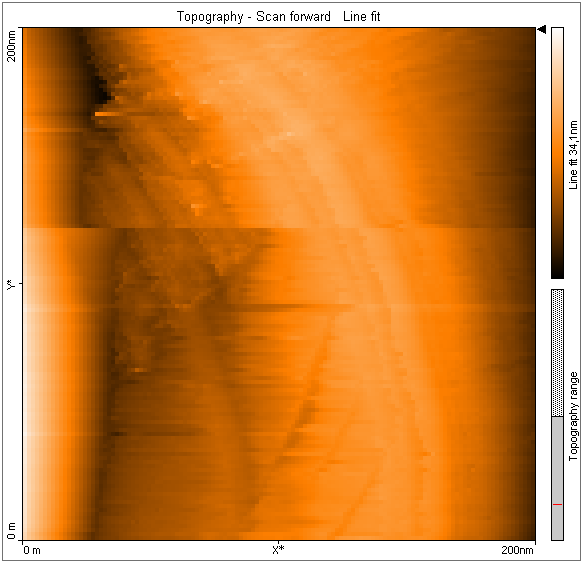
\includegraphics[width=0.6\textwidth]{./grafiken/bohrer.png}
\caption{Bild einer Messung während eine Bohrmaschine im Nebenraum ansprang. Man sieht gut den von der Erschütterung verursachten Versatz der Spitze während der Messung.}
\label{fig:bohrer}
\end{figure}

Als weiterer Störfaktor kommen Erschütterungen von den Maschinen aus dem Nebenraum zustande. Abbildung \ref{fig:bohrer}, die am Ende des zweiten Versuchstages entstand, zeigt dabei gut den Einfluss der Erschütterungen auf die Messung.
Während dieser Datennahme nahm im Nebenraum eine Bohrmaschine den Betrieb auf, was selbst Boden und Tische im Versuchsraum spürbar erschüttern ließ.
Das Bild stellt gleichzeitig auch die beste unserer Messungen dar, leider jedoch nicht mit atomarer Auflösung.

\subsection{Vergleich der Spitzenherstellungsverfahren}

\section{Zusammenfassung}

% BIBLIOGRAPHIE

% Maximale Anzahl der Einträge in Klammer
% Zitieren mit \cite{lamport94}
\begin{thebibliography}{9}

% Beispiel
\bibitem{binning}
  G. Binning et al.,
  \emph{Surface Studies by Scanning Tunneling Microscopy},
  Phys. Rev. Lett. 49, 57 (1982).

\bibitem{colton}
  R. J. Colton, A. Engel, J. E. Frommer et al.,
  \emph{Procedures in Scanning Probe Microscopies},
  John Wiley 1998.

\bibitem{sakai}
  Akira Sakai,
  \emph{Apparent Barrier Height and Barrier-Height Imaging of Surfaces},
  Springer Berlin Heidelberg 2000.
  
\end{thebibliography}

\newpage

\begin{appendix}
\section{Messdaten: Bindungslängen in Graphit}
\label{messw:laenge}
% Table generated by Excel2LaTeX from sheet 'L�nge'
\begin{table}[htbp]
  \centering
    \begin{tabular}{SSSSS}
    \toprule
    {Liniennummer} & {L\"ange $ d / \si{\angstrom}$} &       & {Liniennummer} & {L\"ange $ d / \si{\angstrom}$} \\
    \midrule
    1     & 1,48  &       & 40    & 1,45 \\
    2     & 1,13  &       & 41    & 1,41 \\
    3     & 0,98  &       & 42    & 0,94 \\
    4     & 1,52  &       & 43    & 1,21 \\
    5     & 1,45  &       & 44    & 1,45 \\
    6     & 1,37  &       & 45    & 0,94 \\
    7     & 0,86  &       & 46    & 1,29 \\
    8     & 1,41  &       & 47    & 0,82 \\
    9     & 0,94  &       & 48    & 1,45 \\
    10    & 1,56  &       & 49    & 1,17 \\
    11    & 0,94  &       & 50    & 0,78 \\
    12    & 1,25  &       & 51    & 1,13 \\
    13    & 0,86  &       & 52    & 1,68 \\
    14    & 1,33  &       & 53    & 0,86 \\
    15    & 1,37  &       & 54    & 1,09 \\
    16    & 1,48  &       & 55    & 1,60 \\
    17    & 1,41  &       &       &  \\
    18    & 0,94  &       &       &  \\
    19    & 1,33  &       &       &  \\
    20    & 0,78  &       &       &  \\
    21    & 1,52  &       &       &  \\
    22    & 1,33  &       &       &  \\
    23    & 1,25  &       &       &  \\
    24    & 0,86  &       &       &  \\
    25    & 1,17  &       &       &  \\
    26    & 1,52  &       &       &  \\
    27    & 1,56  &       &       &  \\
    28    & 1,41  &       &       &  \\
    29    & 1,25  &       &       &  \\
    30    & 0,74  &       &       &  \\
    31    & 1,37  &       &       &  \\
    32    & 1,25  &       &       &  \\
    33    & 0,98  &       &       &  \\
    34    & 1,33  &       &       &  \\
    35    & 1,33  &       &       &  \\
    36    &       &       &       &  \\
    37    & 0,86  &       &       &  \\
    38    & 1,25  &       &       &  \\
    39    & 0,86  &       &       &  \\
    \bottomrule
    \end{tabular}%
  \caption{L\"ange der eingezeichneten Linien}
  \label{tab:laengen}%
\end{table}%


\end{appendix}


\end{document}
